\documentclass[aspectratio = 169]{beamer}
%%%%%%%%%%%%%%%%%%%%%%%%%%%%%%%%%%%%%%%%%%%%%%%%%%%%%%%%%%%%%%%%%%%%%%%%%%%%%%%%%%%%%%%%%%%%%%%%%%%%%%%%%%%%%%%%%%%
% Preamble
\usepackage[
    backend = biber,
    style = apa,
    citestyle = authoryear-comp,
    sorting = ydnt,
    mincitenames = 1,
    maxcitenames = 2,
    uniquelist = minyear
]{biblatex}
\addbibresource{emissions.bib}
\AtBeginBibliography{\small}

\usepackage{hyperref}
\hypersetup{colorlinks = true, citecolor = blue, linkcolor = blue, urlcolor = blue, hypertexnames = true}
\newcommand{\shortlink}[1]{\href{https://www.#1}{\texttt{#1}}}

\DeclareCiteCommand{\cite} % Ensures author-year hyperlink applies to \cite
{\usebibmacro{prenote}}
{\usebibmacro{citeindex}%
\printtext[bibhyperref]{\usebibmacro{cite}}}
{\multicitedelim}
{\usebibmacro{postnote}}

\DeclareCiteCommand{\parencite}[\mkbibparens] % Ensures author-year hyperlink applies to \parencite
{\usebibmacro{prenote}}
{\usebibmacro{citeindex}%
\printtext[bibhyperref]{\usebibmacro{cite}}}
{\multicitedelim}
{\usebibmacro{postnote}}

\DeclareCiteCommand{\cite} % Ensures that year appears in parentheses
{\usebibmacro{prenote}}
{\usebibmacro{citeindex}%
\printtext[bibhyperref]{\printnames{labelname} \mkbibparens{\printfield{year}}}}
{\multicitedelim}
{\usebibmacro{postnote}}

% Packages
\usepackage{graphicx} % Required for inserting images
\usepackage{amsmath}
\usepackage{amsfonts}
\usepackage{mathrsfs}
\usepackage{supertabular}
\usepackage{array}
\usepackage{booktabs}
\usepackage{threeparttable}
\usepackage{longtable}
\usepackage{float}
\usepackage{textcomp}
\usepackage{color}
\usepackage{stmaryrd}
%\usepackage{blkarray}

%%%%%%%%%%%%%%%%%%%%%%%%%%%%%%%%%%%%%%%%%%%%%%%%%%%%%%%%%%%%%%%%%%%%%%%%%%%%%%%%%%%%%%%%%%%%%%%%%%%%%%%%%
% Themes
%\usetheme{madrid}
%\usetheme{Warsaw}
%\usetheme{Boadilla}
\usetheme[progressbar = frametitle]{metropolis}
\setbeamertemplate{frame numbering}[fraction]
\metroset{background = dark}

\definecolor{primary}{RGB}{2, 25, 232}
\setbeamercolor{palette primary}{bg = white, fg = black}
\setbeamercolor{background canvas}{parent = palette primary}
\setbeamercolor{normal text}{fg = black}
\setbeamercolor{progress bar}{use = palette primary, fg = primary}

\setbeamercovered{transparent}
%%%%%%%%%%%%%%%%%%%%%%%%%%%%%%%%%%%%%%%%%%%%%%%%%%%%%%%%%%%%%%%%%%%%%%%%%%%%%%%%%%%%%%%%%%%%%%%%%%%%%%%%%
% Title and Authors
\title[]{The Unintended Consequences of Minimum Wage Hikes: Evidence based on Firms' Pollution Emission---Presented by D.O. Ekeocha}

%\author[Ekeocha]{
%    D.O.~Ekeocha\inst{1}
%    \and
%    D.F. ~Giuseppe\inst{1}
%    \and
%    J. ~Lonsky\inst{1}
%}
%\institute[]{
%    \inst{1}
%    University of Liverpool Management School
%    \and
%    \inst{2}
%    SPIRE, University College Dublin
%}
\date{\today}

%%%%%%%%%%%%%%%%%%%%%%%%%%%%%%%%%%%%%%%%%%%%%%%%%%%%%%%%%%%%%%%%%%%%%%%%%%%%%%%%%%%%%%%%%%%%%%%%%%%%%%%%%
% Document
\begin{document}
    \maketitle

    \begin{frame}{Outline}
        \tableofcontents
    \end{frame}


    \section{Objectives \& Main Results}\label{sec:objectives-and-main-results}
    \begin{frame}{Objectives}
        \begin{itemize}
            \item To determine the causal impact of MW hikes on pollution emission intensity of Chinese Manufacturing firms.
        \end{itemize}
    \end{frame}

    \begin{frame}{Main Results}
        \begin{itemize}
            \item MW hike raises firms' pollution emission intensity.
            \item The increase in emission intensity is mainly from inefficient energy consumption, insufficient pollution treatment and failure to upgrade green technologies.
            \item The effect is more pronounced in financially constrained firms, firms in highly competitive and labour-intensive industries but regions with stricter
            environmental regulations exhibit less intensive pollution responses from local firms.
        \end{itemize}
    \end{frame}


    \section{Motivation}\label{sec:motivation}
    \begin{frame}{Motivation---Minimum Wage Policy}
        \begin{itemize}
            \item MW on wages and labour cost---\parencite{coviello2022minimum, alexandre2022minimum}
            \item MW on employment---\parencite{brown1999minimum, neumark1992employment, card2000minimum, cengiz2019effect, dustmann2022reallocation}
            \item MW on consumers---\parencite{harasztosi2019pays}
            \item MW on pollution?
        \end{itemize}
    \end{frame}


    \section{Theoretical Analysis}\label{sec:theoretical-analysis}
    \begin{frame}{Theoretical Analysis}
        \begin{itemize}
            \item There are two competing hypotheses: \textbf{The induced technology change effect and the crowding-out effect.}
        \end{itemize}

        Unintended consequences of a raising minimum wage is an empirical question!

    \end{frame}


    \section{Data \& Identification Strategy}\label{sec:data-and-identification}
    \begin{frame}{Data}
        \begin{itemize}
            \item MW data---county level from $1997$ to $2009$ from Ministry of Human Resources and Social Security.
            \item Pollutant emissions data (chemical oxide demand and sulphur oxide) $1998$ to $2009$---firm level from China's Environmental Statistics Database (CESD) and China's Industrial Enterprise Database (CIED).
            \item Green innovation (green patents) from State's Intellectual Property Office.
            \item Regional macroeconomic variables (GDP and local employment)---county and city level from the Chinese Statistical Year Book.
        \end{itemize}
    \end{frame}

    \begin{frame}{Summary Statistics}
            \begin{figure}
                \centering
                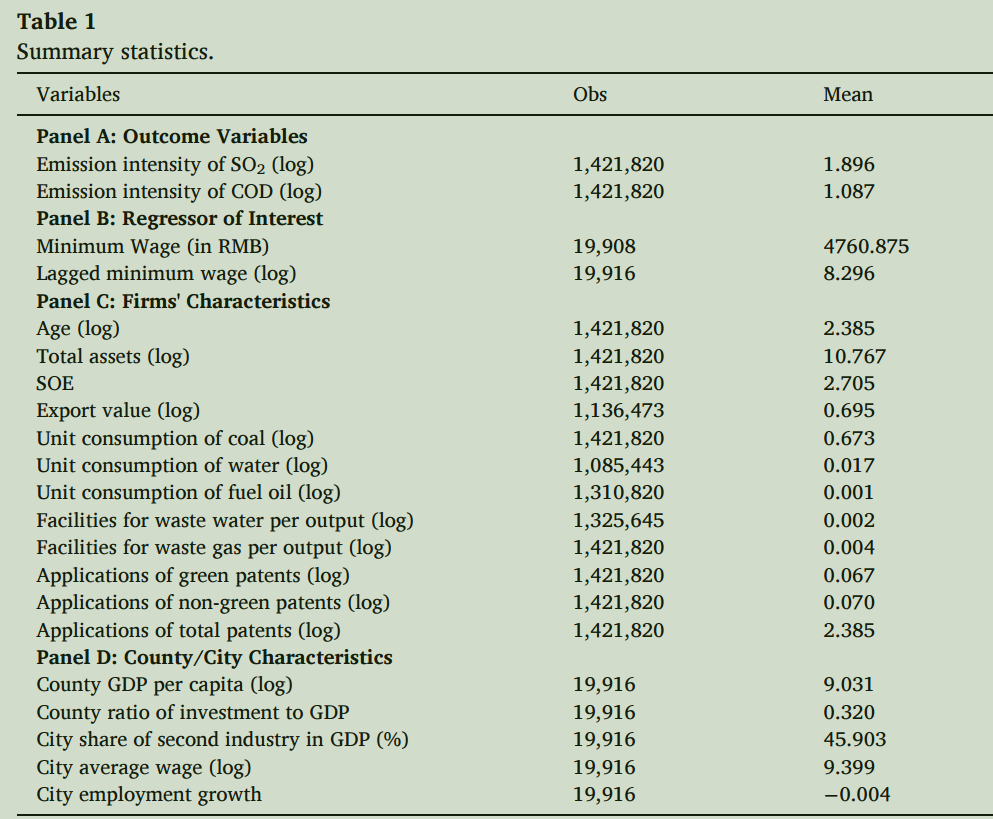
\includegraphics[width = 0.6\textwidth, height = 0.8\textheight]{climate_change/beamer/sumstat}
%                \caption{Evolution of MW in Chinese Counties}
                \label{fig:sumstat}
            \end{figure}
    \end{frame}

    \begin{frame}{Identification Strategy---County Border Discontinuity}
        \begin{itemize}
            \item They leveraged discontinuity in MW policy between adjacent Chinese county pairs at the border~\parencite{dube2010minimum}.
            \item Average MW growth is $9.5\%$.
            \item County pairs must share the same border and range between $50km$, $75km$ and $100km$ away from the border.
            \item Final sample $1,183,702$, $1,214,918$ and $1,217,919$, respectively.
            \item And $89,248$ distinct firms.
        \end{itemize}

    \end{frame}

    \begin{frame}{County Border Discontinuity}
        \begin{columns}
            \column{0.5\textwidth}
            \begin{figure}
                \centering
                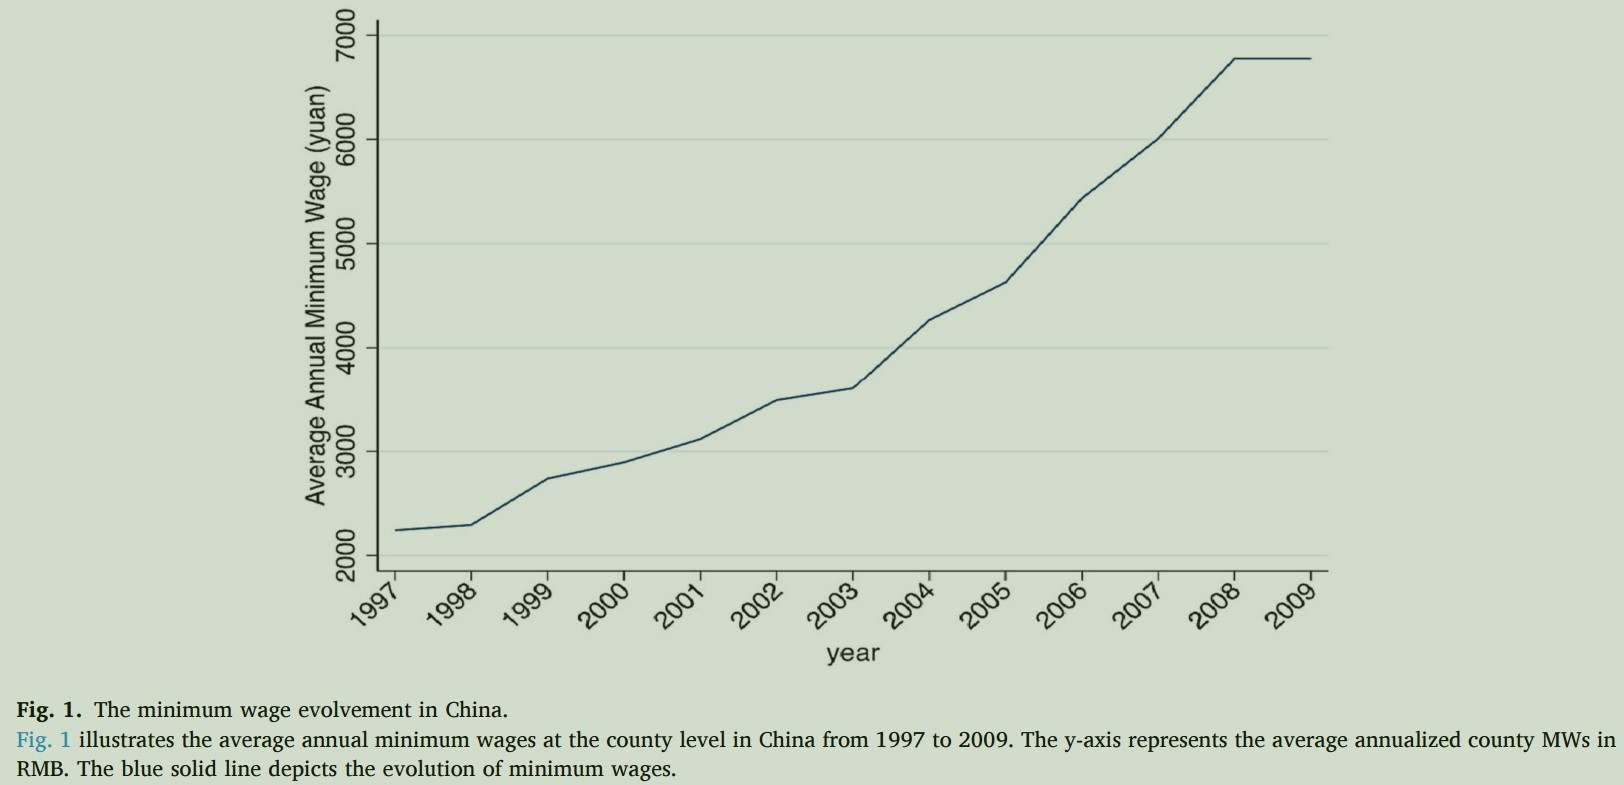
\includegraphics[width = \textwidth, height = 0.6\textheight]{climate_change/beamer/wd}
%                \caption{Evolution of MW in Chinese Counties}
                \label{fig:chinese-mw1}
            \end{figure}

            \column{0.5\textwidth}
            \begin{figure}
                \centering
                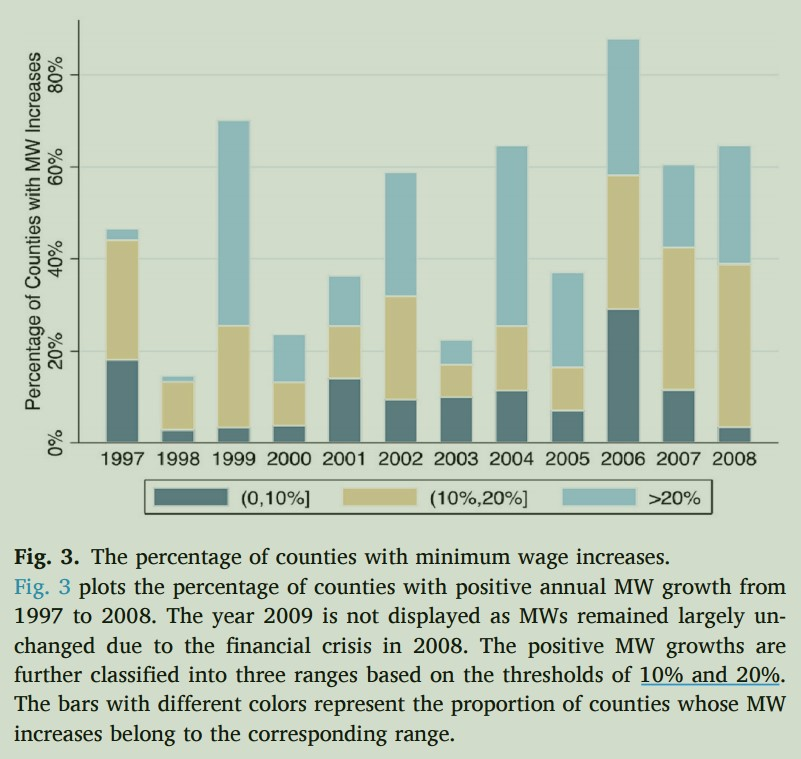
\includegraphics[width = \textwidth, height = 0.7\textheight]{climate_change/beamer/wd2}
%                \caption{Evolution of MW in Chinese Counties}
                \label{fig:chinese-mw2}
            \end{figure}
        \end{columns}
    \end{frame}

%    \begin{frame}[shrink = 25]{Summary Statistics}
%        \input{energy_effects/results/tables/cov.grid.nt.sum.stat}
%    \end{frame}


    \section{Model and Results}\label{sec:model-and-results}
    \begin{frame}{Model}
        \begin{equation}
            ln(MW)_{c,t} = \alpha_0 + \alpha_{1}Determinants_{c,t-1} + \mu_c + \rho_{k,t} + \epsilon_{c,t}\label{eq:determinants-mw}
        \end{equation}

        \begin{equation}
            ln(Pollution)_{i,c,h,p,t} = \beta_{1}ln(MW_{c,t-1}) + \beta_{2}X_{i,t} + \beta_{3}Z_{c,t-1} + \beta_{4}M_{h,t-1} + \theta_{p,t} + \delta_{i} + \epsilon_{i,c,h,p,t}\label{eq:model-mw}
        \end{equation}

        \begin{itemize}
            \item $X_{i,t}$ is the a vector of firm-level characteristics---firm age, ownership, size and export value;
            \item $Z_{c,t-1}$ is a vector of county-level covariates---GDP per capita and capital investments;
            \item $M_{h,t-1}$ is the vector of city-level covariates---share of secondary industry GDP, average wage of urban employees and employment growth rate.
        \end{itemize}
    \end{frame}

    \begin{frame}{Results---MW Determinants}
        \begin{figure}
            \centering
            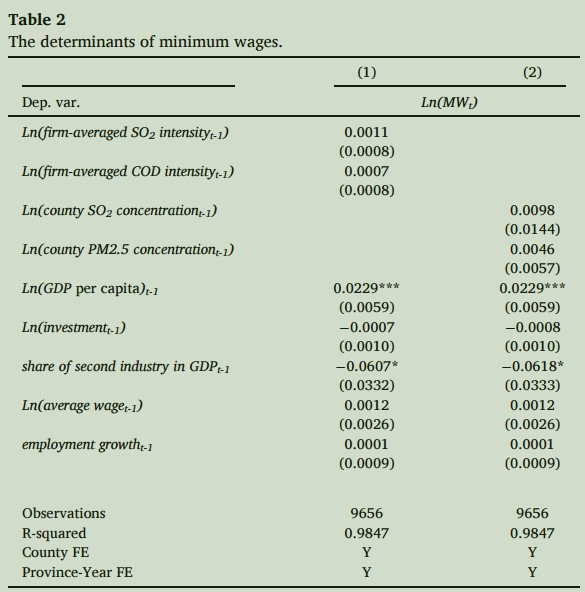
\includegraphics[width = 0.5\textwidth, height = 0.9\textheight]{climate_change/beamer/det}
%                \caption{Evolution of MW in Chinese Counties}
            \label{fig:determinants-mw}
        \end{figure}
    \end{frame}

    \begin{frame}{Results---MW on Wage and Labour Cost}
        \begin{figure}
            \centering
            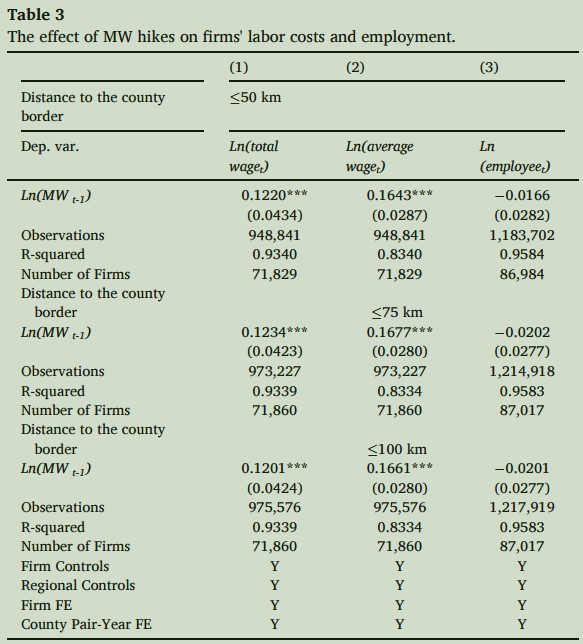
\includegraphics[width = 0.6\textwidth, height = 0.9\textheight]{climate_change/beamer/wage_labor}
%                \caption{Evolution of MW in Chinese Counties}
            \label{fig:wage-labour-mw}
        \end{figure}
    \end{frame}

    \begin{frame}{Plots---MW on Pollution Emission Intensity}
        \begin{columns}
            \column{0.5\textwidth}
            \begin{figure}
                \centering
                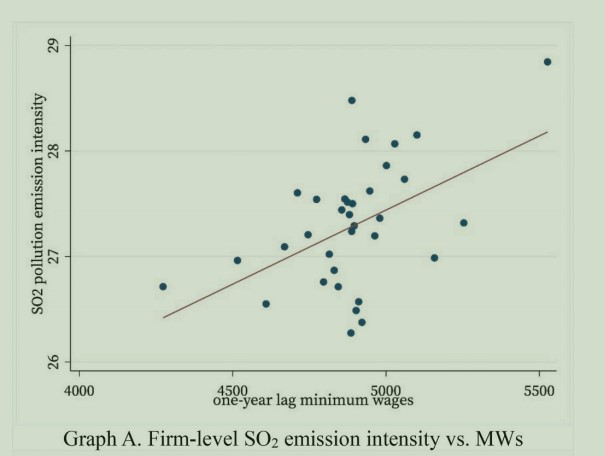
\includegraphics[width = 0.8\textwidth, height = 0.6\textheight]{climate_change/beamer/so2}
%                \caption{Evolution of MW in Chinese Counties}
                \label{fig:so2-mw}
            \end{figure}

            \column{0.5\textwidth}
            \begin{figure}
                \centering
                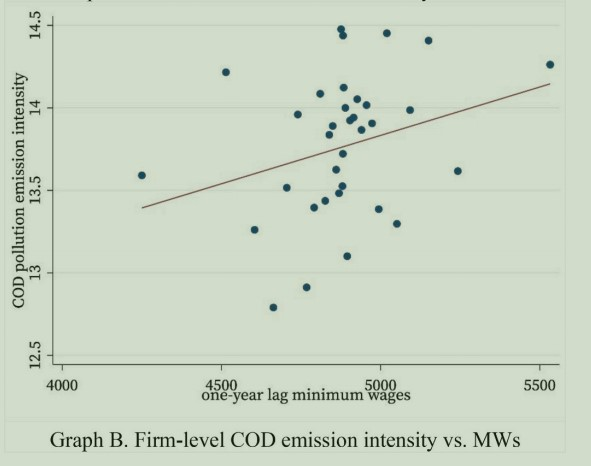
\includegraphics[width = 0.8\textwidth, height = 0.6\textheight]{climate_change/beamer/cod}
%                \caption{Evolution of MW in Chinese Counties}
                \label{fig:cod-mw}
            \end{figure}
        \end{columns}
    \end{frame}

    \begin{frame}{Results---MW on Pollution Emission Intensity}
        \begin{figure}
            \centering
            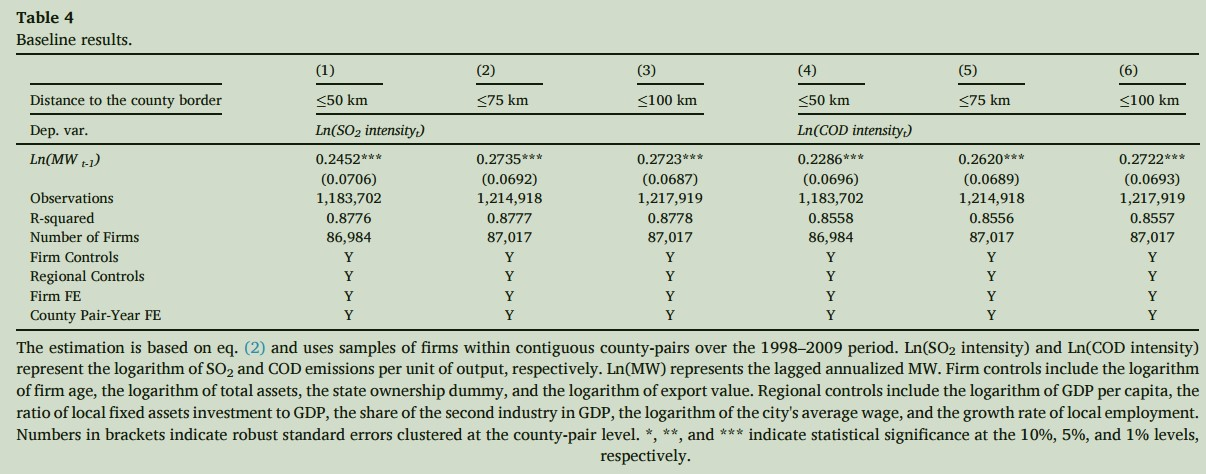
\includegraphics[width = 0.8\textwidth, height = 0.6\textheight]{climate_change/beamer/pol}
%                \caption{Evolution of MW in Chinese Counties}
            \label{fig:pollution-mw}
        \end{figure}
    \end{frame}

    \begin{frame}{Robustness Checks}
        \begin{itemize}
            \item Dropping cross-city county-pairs
            \item Dropping four municipalities---Beijing, Tianjin, Shanghai and Chongqing
            \item Roles of firm entry and exits
            \item Alternative measurements of firms' pollution emission---waste water intensity, waste gas intensity, NOx intensity and Dust intensity.
        \end{itemize}
    \end{frame}

    \begin{frame}{Mechanism Analysis}
        \begin{itemize}
            \item Energy input in the production process---coal, water and fuel oil consumption intensity
            \item End-of-pipe treatment of pollutants---number of waste water treatment facilities per output and number of waste gas treatment facilities per output.
            \item Technological Innovation
        \end{itemize}
    \end{frame}

    \begin{frame}{Hetrogeneity Analysis}
        \begin{itemize}
            \item Financial constraints
            \item High concentrated industries
            \item Environmental regulations
        \end{itemize}
    \end{frame}

    \section{Suggestions}\label{sec:suggestions}
    \begin{frame}{Suggestions}
        \begin{itemize}
            \item Correlation not causality!
            \item This is a Fuzzy RD setup given MW growth across counties---MW intensity.
            \item Restrict the sample to $50km$, $75km$ and $100km$ away from the border.
            \item Define YoY changes in wages from total wages across the periods---$\delta^{w}$.
            \item Create a dummy $D^{w}$ conditional on a running variable---MW that is unity for counties with $\delta^{w} > 0$. These counties will usually be on the other side of the border for all county pairs.
            \item This $D^{w}$ will capture the discontinuity in MW policy at the border and becomes the instrumental variable to recover a causal impact.
        \end{itemize}
    \end{frame}

    \begin{frame}{County Wage Distributions}
        \begin{columns}
            \column{0.33\textwidth}
            \begin{figure}
                \centering
                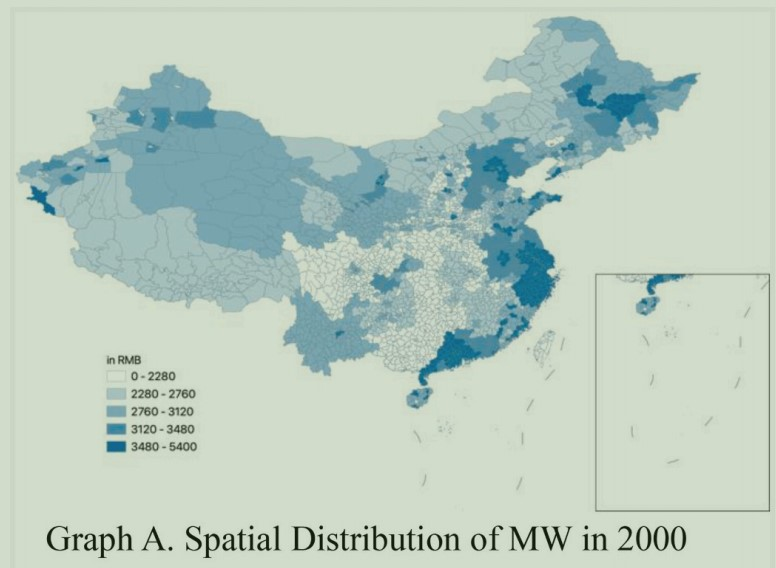
\includegraphics[width = \textwidth, height = 0.5\textheight]{climate_change/beamer/wd2000}
%                \caption{Evolution of MW in Chinese Counties}
                \label{fig:chinese-mw2000}
            \end{figure}

            \column{0.33\textwidth}
            \begin{figure}
                \centering
                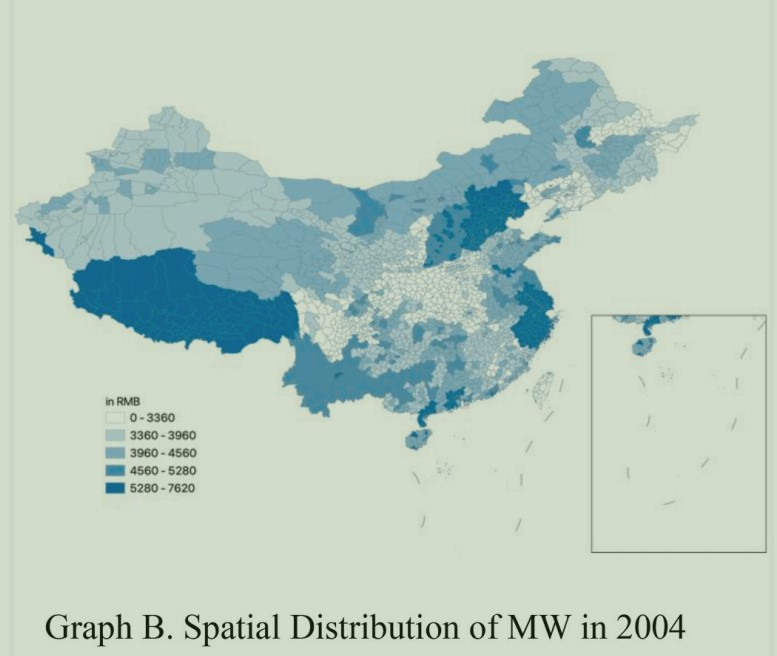
\includegraphics[width = \textwidth, height = 0.5\textheight]{climate_change/beamer/wd2004}
%                \caption{Evolution of MW in Chinese Counties}
                \label{fig:chinese-mw2004}
            \end{figure}

            \column{0.33\textwidth}
            \begin{figure}
                \centering
                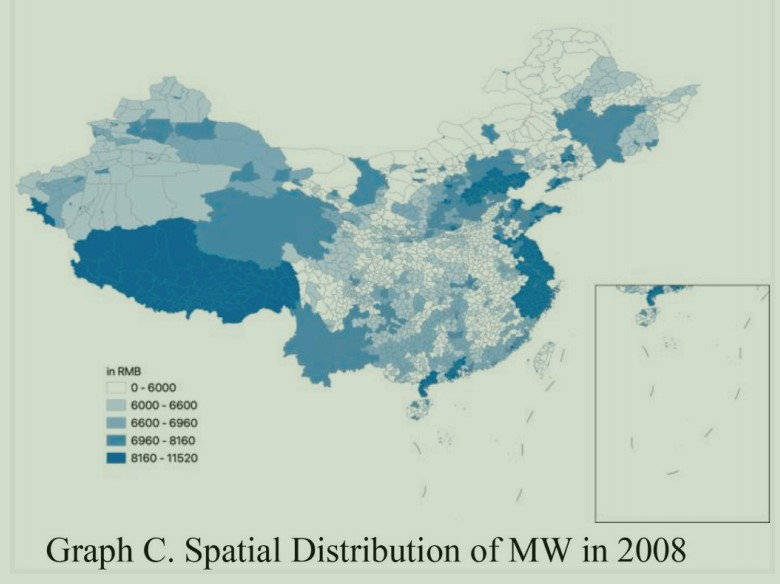
\includegraphics[width = \textwidth, height = 0.5\textheight]{climate_change/beamer/wd2008}
%                \caption{Evolution of MW in Chinese Counties}
                \label{fig:chinese-mw2008}
            \end{figure}
        \end{columns}
    \end{frame}

    \begin{frame}{Suggestions}
        Following equation~\ref{eq:determinants-mw} will be this:
        \begin{equation}
            ln(MW)_{c,t} = \alpha_0 + \alpha_{1}D_{p}^{w} + R_{c,t} + \beta_{4}X_{i,t} + \beta_{5}Controls_{c,h,t-1} + \theta_{p,t} + \delta_{i} + \epsilon_{c,t}\label{eq:first-stage-mw}
        \end{equation}

        \begin{equation}
            ln(Pollution)_{i,c,h,p,t} = \phi ln(\hat{MW}_{c,t}) + R_{c,t} + \beta_{4}X_{i,t} + \beta_{5}Controls_{c,h,t-1} + \theta_{p,t} + \delta_{i} + \epsilon_{i,c,h,p,t}\label{eq:second-stage-mw}
        \end{equation}

        where $R_{c,t} = \beta_{1}\delta_{c,t}^{w} + \beta_{2}ln(MW_{c,t-1}) + \beta_{3}ln(MW_{c,t})^2$
    \end{frame}

    \begin{frame}{Suggestions}
        \begin{itemize}
            \item Estimate baseline equation~\ref{eq:second-stage-mw} for the causal impact measured by $\phi$ for $SO_{2}$ and $COD$.
            \item Estimate equation~\ref{eq:second-stage-mw} separately on either side of the border. That for $D^{w} = 1$ and $D^{w} = 0$.
            \item Plot their fitted values of pollutant emission intensity on MW on the same graph indicating $D^{w}$ as the county border discontinuity MW hikes.
        \end{itemize}
    \end{frame}

%    \begin{frame}{}
%        \centering
%        Thank You for Listening
%    \end{frame}

    \begin{frame}[allowframebreaks, noframenumbering]
        \printbibliography
    \end{frame}

\end{document}